\documentclass[11pt]{article}
\usepackage[margin=1in]{geometry}								% Package to create dummy text
\usepackage{amsmath,amsfonts,amsthm,amssymb}					% Math packages
\usepackage[pdftex]{graphicx}									% Enable pdflatex
\usepackage{hyperref} % URLs
\setlength\parindent{0pt}%noindet-to-whole-document
\newtheorem{thm}{Theorem}[section]
\newtheorem{lem}[thm]{Lemma}
\newtheorem{prop}[thm]{Proposition}
\newtheorem{cor}[thm]{Corollary}
\newtheorem{conj}[thm]{Conjecture}

\theoremstyle{definition}
\newtheorem{defn}[thm]{Definition}
\newtheorem{defns}[thm]{Definitions}
\newtheorem{con}[thm]{Construction}
\newtheorem{exmp}[thm]{Example}
\newtheorem{notn}[thm]{Notation}
\newtheorem{notns}[thm]{Notations}
\newtheorem{addm}[thm]{Addendum}
\newtheorem{exer}[thm]{Exercise}
\newtheorem{rem}[thm]{Remark}
\theoremstyle{plain}



\begin{document}
\nocite{}

\title{Functions}

\author{Miliyon T.}
\date{October 7, 2013}
\maketitle

\section{Introduction}

Millions of years ago, people started noticing that some quantities in nature depend on the others. They studied these dependencies in a chaotic way, and one day they decided enough is enough and they need a unified theory, and that's how the theory of functions started to exist, at least according to history books.

If you think that you already know enough about functions, feel free to scroll to the bottom of this document, and follow the link to a multiple-choice quiz that you can use to test your knowledge.

We will use Cartesian product of sets to define functions in an elegant way. Since it is quite hard to understand the definition when you are seeing it for the first time, we will start by examples of functions and by pointing out the most important properties that the function must satisfy.

We can think of a function as a rule. To each input value we assign exactly one output value according to this rule.

\begin{exmp}
Consider the function \( h:\mathbb N\to\mathbb Z \) defined in the following way: \[ h(x)=x-17.\]
\end{exmp}
This is a function that takes a positive integer as an input and produces an integer as an output. If the input is \( 22 \) then we write \( h(22)=5 \). Let us evaluate this function for several more inputs: \( h(37)=20 \), \( h(100)=83 \), \( h(3)=-14 \). We can represent this graphically as:

\begin{figure}[hbt!]
\centering
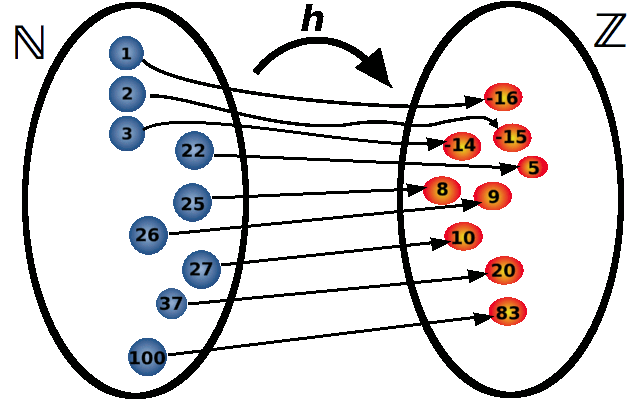
\includegraphics[width=.4\textwidth]{function}
%\caption{ }
\end{figure}

Another way to represent a function is by ordered pairs: \[ (1,-16), (2,-15), (3,-14), \dots, (25,8), (26,9), (27,10), \dots\] The first number in the pair is the input, while the second is the corresponding output. This list of ordered pairs uniquely represents our function \( h \).


\begin{exmp}
Consider the following function \( g:\mathbb N^2\to\mathbb N \): \[ g(x,y)=x+y.\]
\end{exmp}

This function takes an element of \( \mathbb N^2 \). Elements of \( \mathbb N^2 \) are ordered pairs of positive integer. To each positive integer this function assigns its sum. Thus we have \( g(3,17)=20 \), \( g(17,17)=34 \), \( g(11,96)=107 \), etc. We can again write our function \( g \) in a similar way as we did before: \[ \big((1,1),2\big), \big((1,2),3\big), \big((1,3),4\big), \big((1,4),5\big),\dots \] \[ \big((2,1),3\big), \big((2,2),4\big), \big((2,3),5\big), \big((2,4),6\big),\dots \] \[ \big((3,1),4\big), \big((3,2),5\big), \big((3,3),6\big), \big((3,4),7\big),\dots \]
\[ \dots\dots\dots\]

Consider the first element in the list: \( \big ((1,1),2\big) \). This is one ordered pair. Its second component is 2. Its first component is another ordered pair: \( (1,1) \). The entire thing \( \big ((1,1),2\big) \) means that if the input is \( (1,1) \) the output is \( 2 \).

\section{Function}

\begin{defn}[Function]
If \( X \) and \( Y \) are two sets, any subset \( f\subseteq X\times Y \) is called a function from \( X \) to \( Y \) if it satisfies the following condition:

For every \( x\in X \) there exists exactly one \( y\in Y \) such that \( (x,y)\in f \).
\end{defn}

The set \( X \) is called domain of function. The set \( Y \) is called co-domain (or range).

Every function is given by its domain, co-domain, and some rule describing how elements from domain are mapped to the co-domain.

\subsection{Image and pre-image of a function}

Assume that \( f:X\to Y \) is a function.

Assume that \( A\subseteq X \). We define the image of \( A \) (and denote it by \( f(A) \)) in the following way: \[ f(A)=\left\{ f(x): x\in A\right\}.\]
Consider the function \( h \) from Example 1. Then we have \[ h\left(\{3,25\}\right)=\{-14,8\}, h\left(\{5,17,35\}\right)=\{-12,0,18\}.\]

Assume that \( B\subseteq Y \). We define the pre-image of \( B \) (and denote it by \( f^{-1}(B) \) as the set of all elements from \( X \) that get mapped to \( B \). The precise definition is the following: \[ f^{-1}(B)=\left\{x\in X: f(x)\in B\right\}.\]
Again, consider the function \( h \) from Example 1. \[ h^{-1}\left(\{7,8,11)\}\right)=\{24,25,38\},\;\; h^{-1}\left(\{-5\}\right)=\{12\},\;\; h^{-1}\left(\{-33\}\right)=\emptyset.\]

The experience has shown that you have a better chance of remembering the following theorem if it is stated in a rather unconventional way, as a multiple-choice question.

%Pre-image ABCD question
\begin{exer}
Assume that \( P \) and \( Q \) are two sets. Then one of the following propositions is false, while the others are true. Prove those that are true, and find a counter-example for the false one.

(A) \( f(P \cup Q)=f(P)\cup f(Q) \).

(B) \( f(P\cap Q)=f(P)\cap f(Q) \).

(C) \( f^{-1}(P \cup Q)=f^{-1}(P)\cup f^{-1}(Q) \).

(D) \( f^{-1}(P\cap Q)=f^{-1}(P)\cap f^{-1}(Q) \).
\end{exer}
\begin{proof}[Solution.]
(A) This is true. We need to prove the following two relations: \[ f(P\cup Q)\subseteq f(P)\cup f(Q)\;\;\mbox{ and }f(P\cup Q)=f(P)\cup f(Q).\] For the first one, assume that \( x\in P\cup Q \), Then we have \( x\in P \) or \( x\in Q \). Assuming that \( x\in P \) we conclude that \( f(x)\in f(P) \) hence the first relation holds.

For the second one, assume that \( y\in f(P)\cup f(Q) \). Then we have \( y\in f(P) \) or \( y\in f(Q) \). Wihtout loss of generality, assume that the first relation holds, we have that \( y=f(x) \) for some \( x\in P \) and since this \( x \) must belong to \( P\cup Q \) we have \( y\in f(P\cup Q) \).

(B) This is the false one!!! We can build quite simple counter example. Let \( X=Y=\{0,1\} \) and let \( f:X\to Y \) be defined as \( f(0)=1 \) and \( f(1)=1 \). Take now \( P=\{0\} \) and \( Q=\{1\} \). Then \( P\cap Q=\emptyset \) and \( f(P\cap Q)=0 \). On the other hand, we have \( f(P)\cap f(Q)=\{1\}\cap \{1\}=\{1\} \).

(C) This is true. If \( x\in f^{-1}(P\cup Q) \) then \( f(x)\in P\cup Q \). We must have \( f(x)\in P \) or \( f(x)\in Q \). Without loss of generality assume that \( f(x)\in P \). Then we have that \( x\in f^{-1}(P) \) hence \( x\in f^{-1}(P)\cup f^{-1}(Q) \). We established the relation \( f^{-1}(P\cup Q)\subseteq f^{-1}(P)\cup f^{-1}(Q) \).

For the reverse inclusion, we assume that \( x\in f^{-1}(P)\cup f^{-1}(Q) \). Assume further that \( x\in f^{-1}(P) \). Then \( f(x)\in P\subseteq P\cup Q \) hence \( x\in f^{-1}(P\cup Q) \).

(D) This proposition is true. Assume that \( x\in f^{-1}(P\cap Q) \). Then \( f(x)\in P\cap Q \) which implies that \( f(x)\in P \) and \( f(x)\in Q \). Therefore \( x\in f^{-1}(P) \) and \( x\in f^{-1}(Q) \). Hence \( x\in f^{-1}(P)\cap f^{-1}(Q) \). This proves that \[ f^{-1}(P\cap Q)\subseteq f^{-1}(P)\cap f^{-1}(Q).\] For the reverse inclusion, we assume that \( x\in f^{-1}(P)\cap f^{-1}(Q) \). Then we have \( x\in f^{-1}(P) \) and \( x\in f^{-1}(Q) \). This implies that \( f(x)\in P \) and \( f(x)\in Q \), therefore \( f(x)\in P\cap Q \) and \( x\in f^{-1}(P\cap Q) \).
\end{proof}

\subsection{Injective, surjective, and bijective functions}

\begin{defn}[Injective functions]
A function \( f:X\to Y \) is called one-to-one (or injective) if: \[ x_1,x_2\in X\mbox{ and } f(x_1)=f(x_2) \;\;\Rightarrow \;\; x_1=x_2.\]
\end{defn}

In other words no two different values from \( X \) are mapped to the same value in \( Y \).

\begin{defn}[Surjective functions]
A function \( f:X\to Y \) is called onto (or surjective) if for every \( y\in Y \) there exists \( x\in X \) such that \( f(x)=y \).
\end{defn}
\begin{defn}[Bijective functions]
A function \( f:A\to B \) is called bijective if it is both one-to-one and onto.
\end{defn}

\begin{defn}[Composition of functions]
Assume that \( f:X\to Y \) and \( g:Y\to Z \) are two functions. We define their composition \( g\circ f \) as a function \( g\circ f:X\to Z \) in the following way: For \( x\in X \) we have: \[ g\circ f(x)= g\big(f(x)\big).\]
\end{defn}

\begin{thm}
Assume that \( f:X\to Y \) and \( g:Y\to Z \) are two functions. Then the following statements are true:

(a) If \( f \) and \( g \) are injective, then so is \( g\circ f \);

(b) If \( f \) and \( g \) are surjective, then \( g\circ f \) is surjective;

(c) If \( g\circ f \) is injective, then \( f \) is injective;

(d) If \( g\circ f \) is surjective, then \( g \) is surjective.
\end{thm}
\begin{proof}
(a) Assume that \( g(f(x))=g(f(x^{\prime})) \) for \( x,x^{\prime},\in X \). Since \( g \) is injective we immediately conclude that \( f(x)=f(x^{\prime}) \). From the injectivity of \( f \) we now get \( x=x^{\prime} \). Hence \( g\circ f \) is injective.

(b) Assume that \( z\in Z \). Since \( g \) is surjective there is \( y\in Y \) such that \( g(z)=y \). Since \( f \) is surjective then there is \( x\in X \) that satisfies \( f(x)=y \). We now have \( g\circ f(x)=g(f(x))=g(y)=z \).

(c) Assume that \( f(x)=f(x^{\prime}) \). We now have that \( g(f(x))=g(f(x^{\prime})) \), or, equivalently that \( g\circ f(x)=g\circ f(x^{\prime}) \). This implies that \( x=x^{\prime} \) Hence \( f \) is injective.

(d) Assume that \( z\in Z \). Since \( g\circ f \) is surjective, there exists \( x\in X \) such that \( g\circ f(x)=z \). However, this means that for \( y=f(x) \) we have \( g(y)=g(f(x))=z \). Thus \( g \) is surjective.
\end{proof}

If a function \( f:X\to Y \) is bijective then it has an inverse. In other words, there exists a bijective function \( g:Y\to X \) such that \( g(f(x))=x \) for all \( x\in X \). Then we have \( g(f(y))=y \) for all \( y\in Y \).

The inverse of a function is denoted by \( f^{-1} \).

You may have noticed that the symbol \( f^{-1} \) is already used in this page. We used it to denote the pre-image of a set. Pre-image of the set exists always, while the inverse is a privilege of bijective functions only. From the context it is usually clear what we mean when we write \( f^{-1}( \) something\( ) \). For example, if that ''something'' is a set, we mean the pre-image. If it is a number we are talking about inverse function.

\end{document} 